\section{Classification} \label{sec:classfication}

We addressed the problem of mapping a workload to a standard benchmark class
using two techniques.

\subsection{Clustering}
\label{sec:clustering}

Clustering was our first approach as an unsupervised algorithm seemed to best
fit the data at hand.
We evaluated the following clustering algorithms in Scikit.\\

\begin{itemize}
\item \textbf{K-Means} :
This algorithm clusters the samples into groups of similar variance by
minimizing the within-cluster sum-of-squares. The number of clusters
needs to be specified. The algorithms scales well to a large number of
samples.

Given a set of $n$ samples X, the algorithm splits them into $K$ disjoint
clusters, wherein each cluster is defined by the mean $\mu_k$ of the samples in
the cluster i.e. the centroids of the cluster.
The algorithm minimizes the within-cluster sum-of-squares criterion:
$$\sum_{i=0}^{n}\min_{\mu_{k} \in C}(\| x_{k} - \mu_{i} \|^2)$$\\

\item \textbf{Affinity Propagation}:
This algorithm creates clusters by passing messages between pairs of samples
till it reaches convergence. The clusters are described using a small number of
exemplars that are most representative of the dataset.
The messages indicate the suitability of one sample to be the exemplar of the
other and this gets updated over time for the entire dataset.

For a pair of samples $i$ and $k$, the evidence that sample $k$ should be the
exemplar for sample $i$ is defined by:
$$r(i,k) \leftarrow s(i,k) - max [a(i,j) + s(i,j) \forall j\neq k ]$$

Here, $s(i, k)$ is a similarity metric and availability $a(i, k)$ is the
accumulated evidence that sample $i$ should choose sample $k$ as its exemplar.
Thus, the exemplars chosen are similar enough to many samples and are
chosen by many samples to be representative of themselves.\\

\item \textbf{Mean-Shift} :
This algorithm tries to identify blobs in a smooth density of samples.
It works by first identifying candidates for centroids and then filtering them
to eliminate near-duplicates.

For a candidate centroid $x_i$ in iteration $t$, the algorithm updates
the candidate effectively to be the mean of the samples within its neighborhood:

$$x_{i}^{t+1} = x_{i}^{t} + \frac{\sum_{x_{j} \in N(x_i)}K(x_{j} -
x_{i})x_{j}}{\sum_{x_{j} \in N(x_{i})}K(x_{j} - x_{i})} $$

Here, $N(x_i)$ depicts the neighborhood of samples within a given distance
around $x_i$ and the additive term is basically the mean shift vector
computed for each centroid that points towards a region of the maximum
increase in the density of points.\\

\begin{figure*}[h!]
    \centering
    \fbox{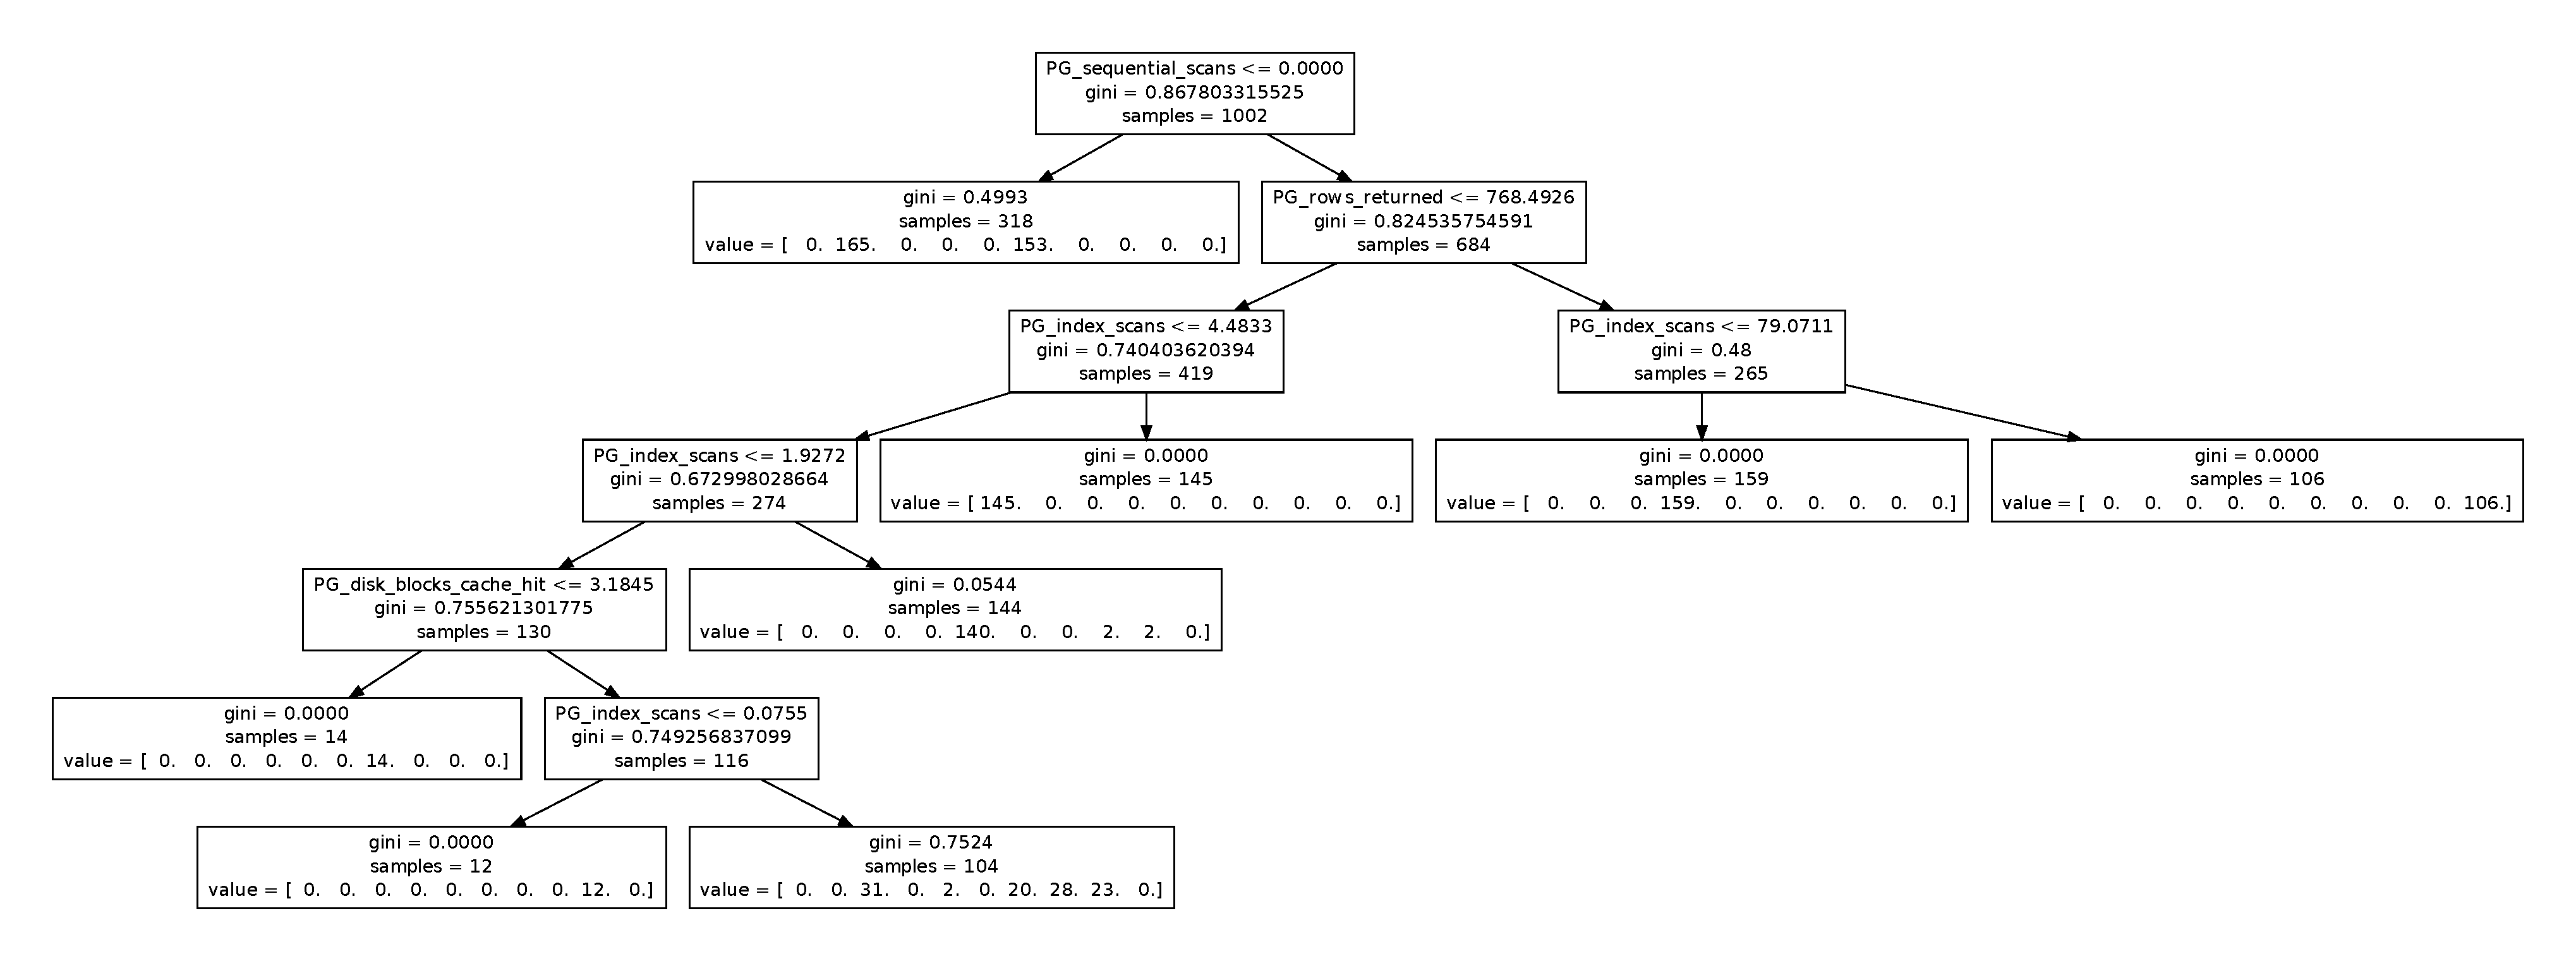
\includegraphics[width=\linewidth]{figure/tree_leaves_8.pdf}}
    \caption{Decision tree with max number of leaves set to 8.}
    \label{fig:tree_sample}
\end{figure*}

\begin{figure}[h!]
    \centering
	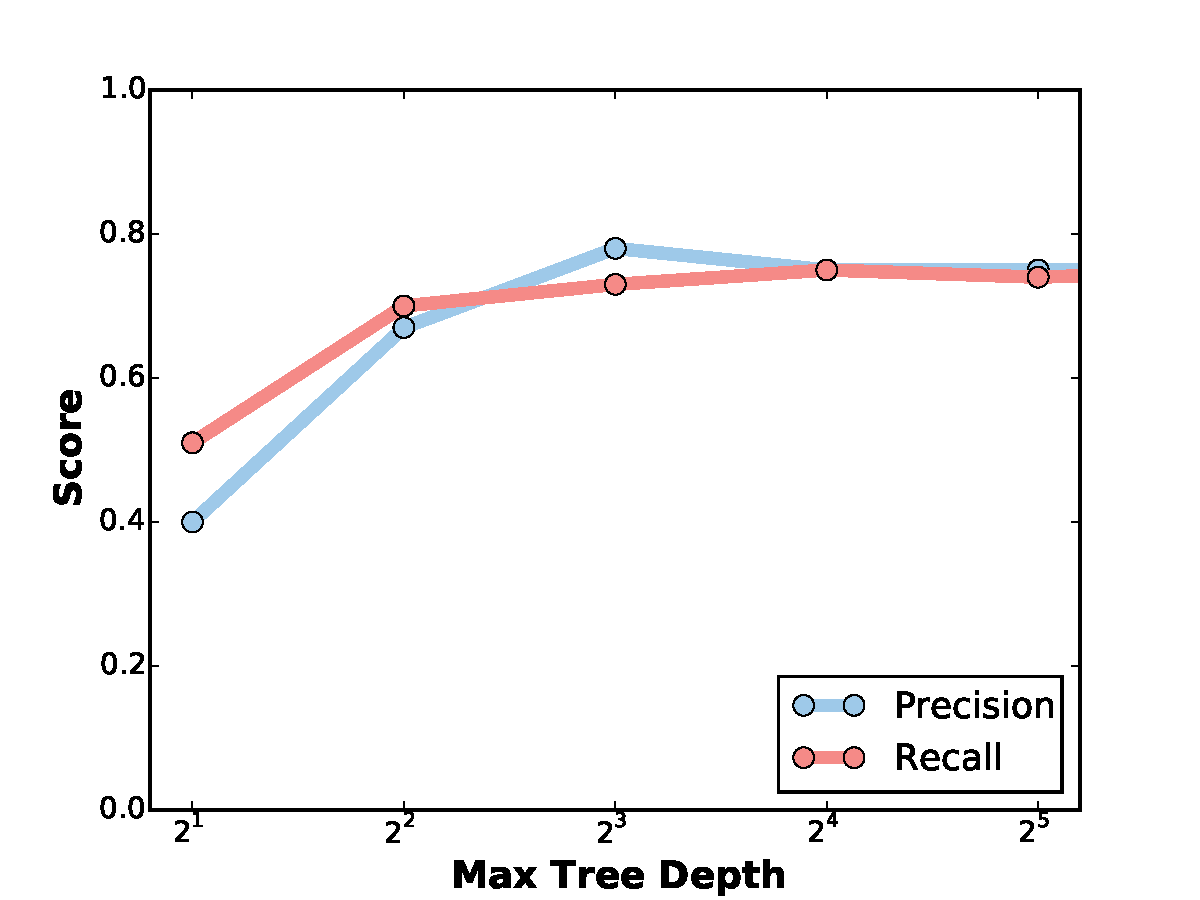
\includegraphics[width=0.7\linewidth]{figure/depth.pdf}
	\caption{Impact of max depth on the accuracy of the decision tree.}
	\label{fig:tree_depth}
\end{figure}

\begin{figure}[h!]
    \centering
	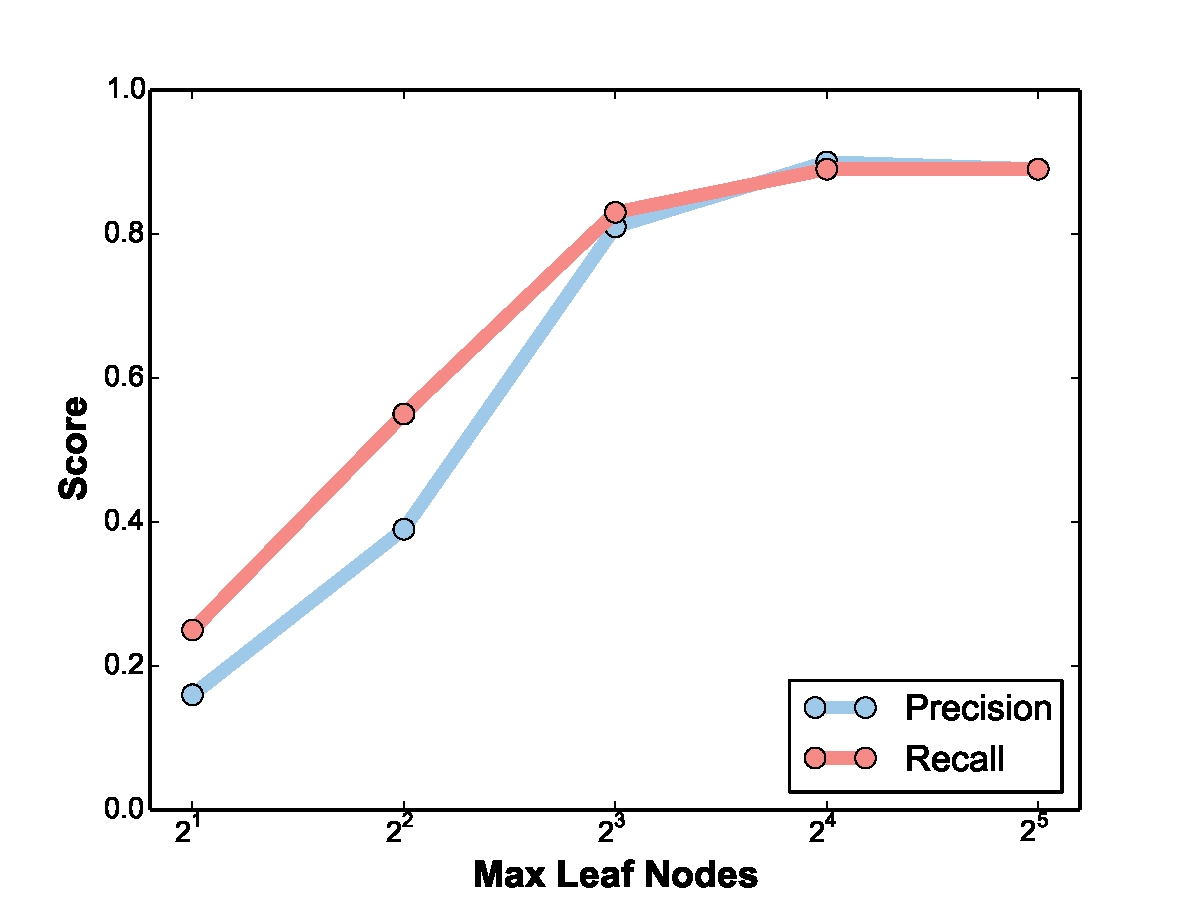
\includegraphics[width=0.7\linewidth]{figure/leaves.pdf}
	\caption{Impact of max leaf nodes on the accuracy of the decision tree.}
	\label{fig:tree_leaves}
\end{figure}

\item \textbf{Agglomerative Clustering} :
This algorithm is a type of hierarchical clustering algorithms that build nested clusters
by merging or splitting them successively.
The cluster hierarchy is represented as a tree, wherein the root is the unique
cluster that gathers all the samples and the leaves are the clusters with only
one sample.
This particular algorithm uses a bottom up approach. Each samples starts in
its own cluster, and over time the clusters are successively merged together
based on a linkage criteria.
We use the \textit{ward} criteria that minimizes the sum of squared differences
within all clusters that is effectively a variance-minimizing approach.
\end{itemize}

The clusters found by each algorithm in high-dimensional space are shown in
\cref{fig:clusters}.
We computed standard clustering metrics for each algorithm including the
following :\\

\begin{itemize}
  \item \textbf{Homogeneity}:
	Given a ground truth, this metric computes if all the clusters contain only
	data points which are members of a single class.\\

  \item \textbf{Completeness}:
	Given a ground truth, this metric computes if all the data points that are
	members of a given class are elements of the same cluster.\\

  \item \textbf{V-measure}:
	This metric is the harmonic mean between homogeneity and completeness
	\citep{v-measure}.

	$$v = 2 * \frac{(homogeneity * completeness)}{(homogeneity + completeness)}$$\\

  \item \textbf{Silhouette coefficient}:
  This metric is computed using the mean intra-cluster distance
  $a$ and the mean nearest-cluster distance $b$ for each sample.
  It is defined for each sample as $(b-a)/max(a, b)$.\\
\end{itemize}

These results are presented in \cref{fig:clustering-metrics}. We observe that
the clustering algorithms work reasonably well with our dataset
especially the K-Means and Ward Agglomerative Clustering algorithms.
Both these algorithms require number of clusters as a parameter.
However, this is not a restriction for our problem as we know the number of
benchmarks - and hence the number of clusters - that we have.
Algorithms like Affinity-Propagation and Mean-Shift give very high and
very low estimates for the number of clusters in the dataset respectively.
As we required higher classification accuracy and better intuition about
the classifier, we also experimented with SVM classifiers and decision trees.
We finally decided to use decision trees as they met both our accuracy
and intuition requirements.

\begin{figure*}
\centering
\subfloat[\label{fig:gp_r2_latency}]{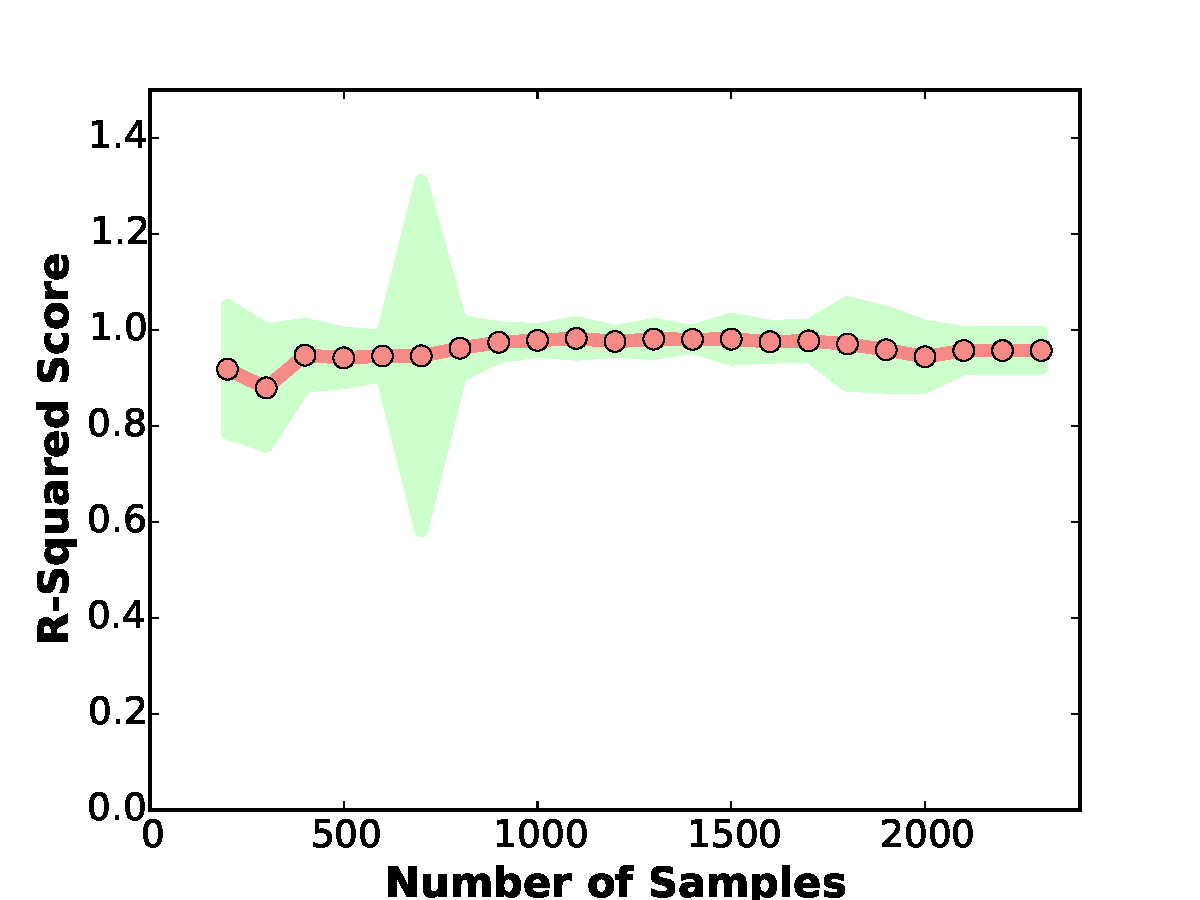
\includegraphics[width=0.4\textwidth]{figure/gp_per_benchmark_r2_scores_latency_mutate.pdf}}
%
\subfloat[\label{fig:gp_r2_throughput}]{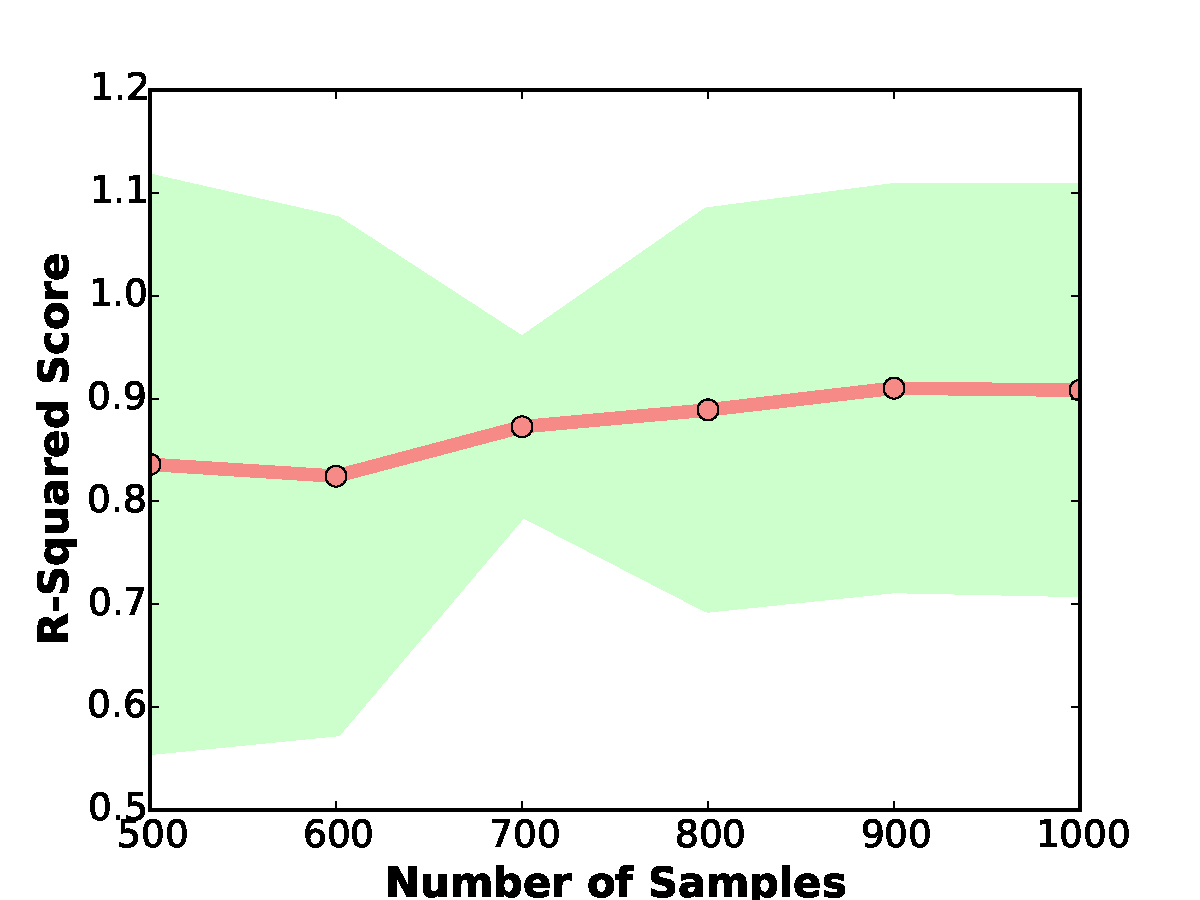
\includegraphics[width=0.4\textwidth]{figure/gp_per_benchmark_r2_scores_throughput_mutate.pdf}}

\caption{Per-benchmark gaussian processes to estimate (a) latency and
  (b) throughput}
\label{fig:gp_r2}
\end{figure*}


\subsection{Decision Trees}
\label{sec:dt}

Decision trees are non-parametric supervised learning algorithms used for
both classification and regression.
It creates a model for predicting the class of a sample by learning
simple decision rules inferred from the sample features\citep{stats01}.
These trees can be interpreted easily and visualised.
We however need to be careful not to create overly complex trees
that do not generalise the data well, i.e. we should avoid overfitting.

Given a set of training samples $x_i \in R^n$, $i=1,...,l$ and the
corresponding label vector $y \in R^l$, the decision tree partitions
the space recursively so that samples with the same labels are grouped
together.
We denote the data at a node $m$ in the decision tree as $Q$. For
every candidate split $\theta = (j, t_m)$ that consists of a feature $j$
and a feature-specific threshold $t_m$, the tree partitions the data into
two subsets $Q_{left}(\theta)$ and $Q_{right}(\theta)$, wherein :
$$Q_{left}(\theta) = {(x, y) | x_j <= t_m}$$
$$Q_{right}(\theta) = Q \setminus Q_{left}(\theta)$$

At each node $m$, we compute an impurity measure that we denote by $H$.
$$G(Q,\theta) = \frac{n_{left}}{N_m} H(Q_{left}(\theta)) +
\frac{n_{right}}{N_m} H(Q_{right}(\theta))$$

We search for parameters that minimize $H$:
$$\theta^* = \operatorname{argmin}_\theta G(Q,\theta)$$

We then do the same process recursively for subsets $Q_{left}(\theta^*)$ and
$Q_{right}(\theta^*)$ until we reach the maximum allowable depth or $N_m
< \min_{samples}$ or $N_m = 1$.
For the classification problem where the target is in $[ 0, K-1]$
for node $m$, representing a region $R_m$ with $N_m$ observations,
the proportion of class $k$ observations in node $m$ is given by :
$$p_{mk} = 1/ N_m \sum_{x_i \in R_m} I(y_i = k)$$
We use the \textit{Gini measure} as the impurity measure:
$$H(X_m) = \sum_k p_{mk} (1 - p_{mk})$$

The implementation uses an optimized version of the CART (Classification and
Regression Trees) algorithm\citep{cart84}.
It basically constructs binary trees using the feature and threshold that
yield the largest information gain at each node.
The features need not be categorical as the algorithm dynamically
defines a discrete attribute based on numerical variables that
partitions the continuous attribute value into a discrete set of intervals.
It does not compute rule sets unlike the C4.5 algorithm\citep{quinlan93}.

A sample decision tree with maximum depth limited to $4$ is shown in
\cref{fig:tree_sample}. We obtain $76\%$ accuracy with this short tree.
The per-class accuracy metrics of the decision tree is shown in
\cref{tab:dt_stats}.
The precision is the ratio $tp/(tp+fp)$ where $tp$ is the number of true
positives and $fp$ the number of false positives.
It is intuitively the ability of the classifier not to label
as positive a sample that is negative.
The recall is the ratio $tp/(tp+fn)$ where $tp$ is the number of true
positives and $fn$ the number of false negatives. It is intuitively the
ability of the classifier to find all the positive samples.
The F1 score is a weighted average of the precision and recall
and is defined as:
$$F1 = 2 * \frac{(precision * recall)}{(precision + recall)}$$
The support is the number of occurrences of each class in the true label
vector $y\_true$.

These are some interesting observations derived from the decision tree shown in
\cref{fig:tree_sample}:\\

\begin{itemize}
  \item Wikipedia benchmark performs a lot of index scans.
  \item SEATS benchmark involves fetching several rows per transaction.
  \item Epinions benchmark, on the other hand, involves returning several rows
  per transaction.
  \item Auctionmark benchmark has less locality of reference i.e. the number of
  disk block cache hits is low.
  \item Twitter benchmark also fetches several rows per transaction. However, it
  does not perform any sequential scans.\\
\end{itemize}

\begin{figure*}
\centering
\subfloat[\label{fig:actual_latency_wikipedia}]{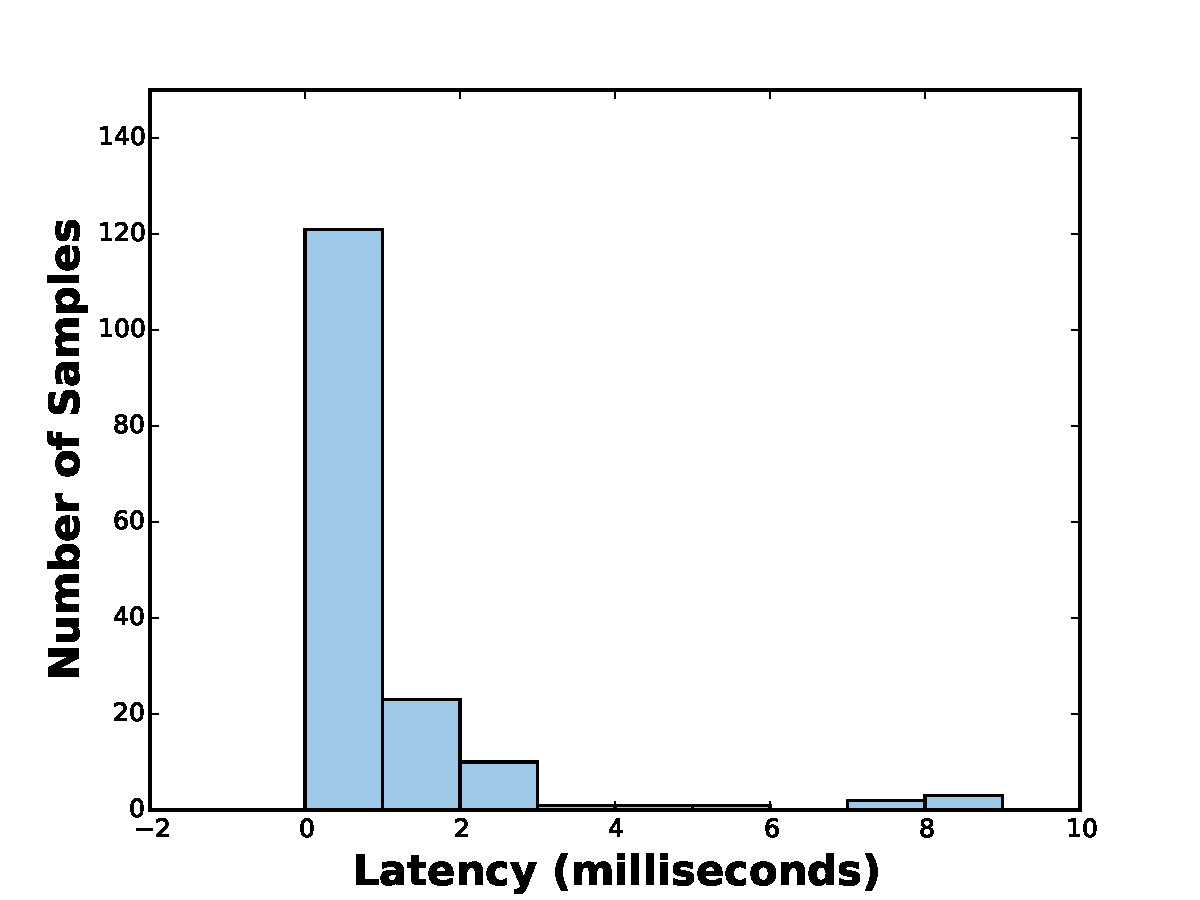
\includegraphics[width=0.4\linewidth]{figure/wikipedia_test_hist_latency_mutate.pdf}}
\subfloat[\label{fig:predicted_latency_wikipedia}]{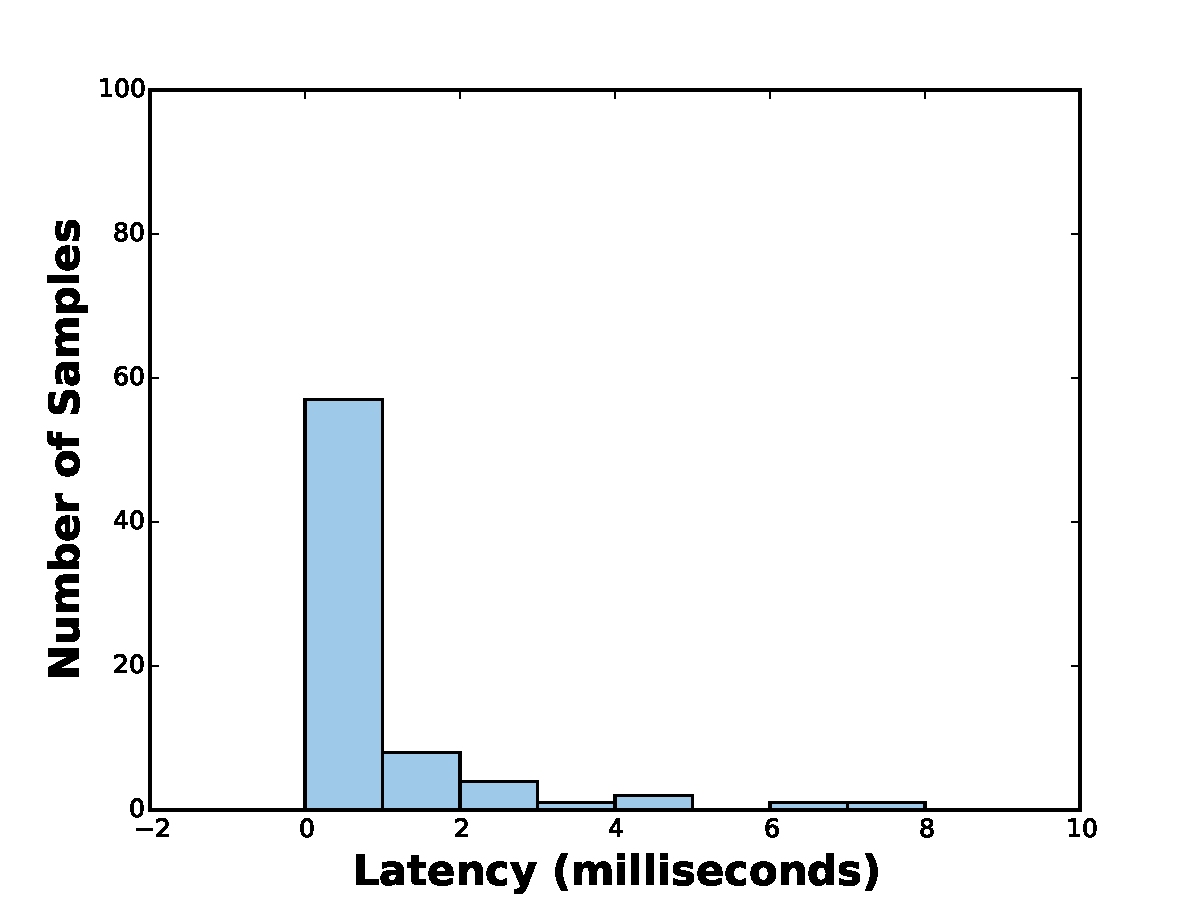
\includegraphics[width=0.4\linewidth]{figure/wikipedia_pred_hist_latency_mutate.pdf}}

\caption{(a) Actual and (b) predicted latency distribution for the
  Wikipedia benchmark}
\label{fig:latency_wikipedia}
\end{figure*}

\begin{figure*}
\centering
\subfloat[\label{fig:actual_throughput_ycsb_balanced}]{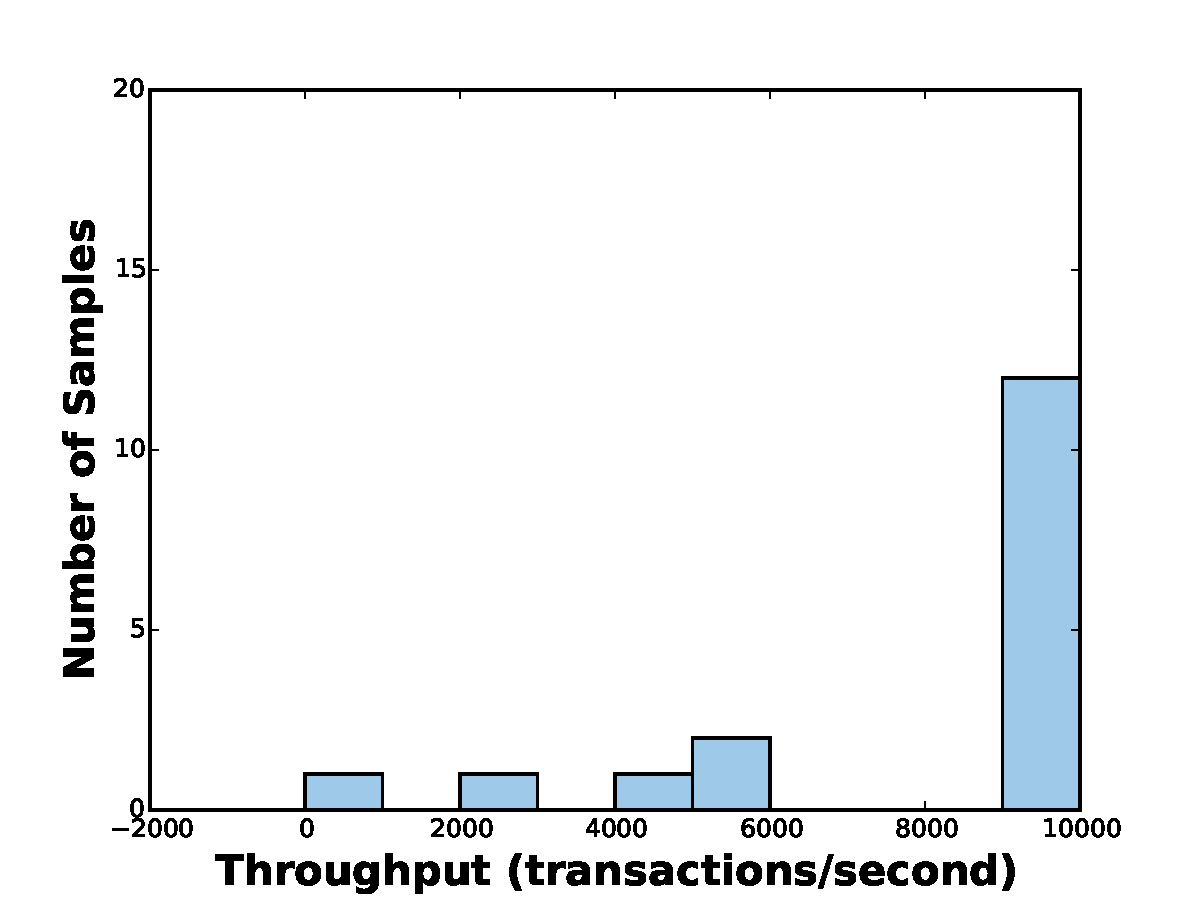
\includegraphics[width=0.4\linewidth]{figure/ycsb_balanced_test_hist_throughput_mutate.pdf}}
\subfloat[\label{fig:predicted_throughput_ycsb_balanced}]{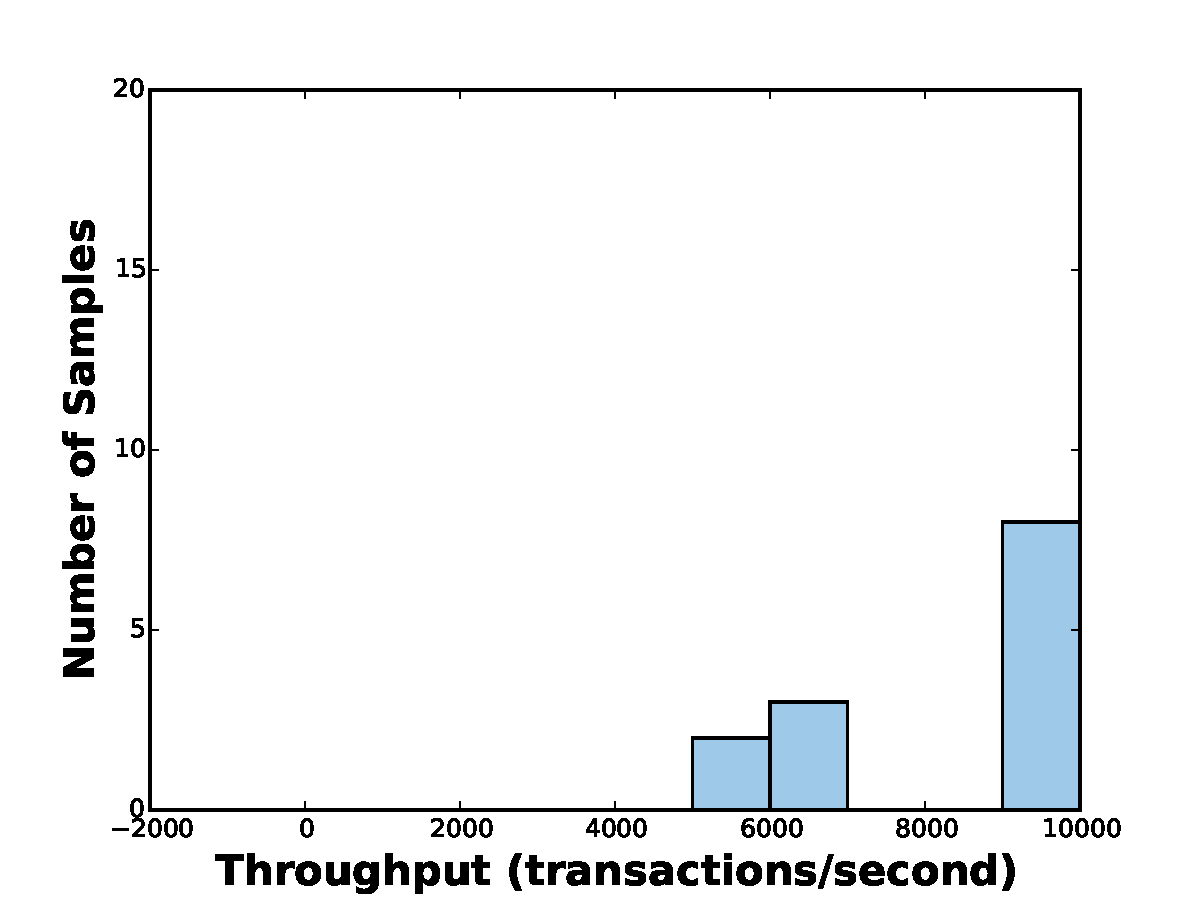
\includegraphics[width=0.4\linewidth]{figure/ycsb_balanced_pred_hist_throughput_mutate.pdf}}

\caption{(a) Actual and (b) predicted throughput distribution for the
  balanced YCSB benchmark}
\label{fig:throughput_ycsb_balanced}
\end{figure*}


The accuracy increases quickly to $91\%$ with a maximum depth of $8$. The impact
of maximum tree depth on the accuracy of the decision tree classifier
is presented in \cref{fig:tree_depth}. Using three-way cross validation,
we verified that the tree is able to classify the dataset accurately
without overfitting.
The impact of maximum number of leaf nodes on the accuracy of the
decision tree classifier is presented in \cref{fig:tree_leaves}.
We observe that these parameters affect both precision and recall
equally. The accuracy increases more steeply with increasing tree
depth as expected.

\begin{table}[h!]
  \centering
  \begin{tabular}{l|llll}
	\toprule
   		Class &  Precision  &  Recall &  F1-score  &  Support  \\
    \midrule
		0.0   &    1.00   &   0.00   &   1.00   &     84   \\
        1.0   &    0.99   &   1.00   &   0.99   &     74   \\
        2.0   &    0.98   &   0.99   &   0.98   &     81   \\
        3.0   &    0.54   &   0.39   &   0.45   &     18   \\
        4.0   &    1.00   &   1.00   &   1.00   &     69   \\
        5.0   &    1.00   &   0.99   &   0.99   &     70   \\
        6.0   &    1.00   &   0.95   &   0.97   &     60   \\
        7.0   &    0.41   &   0.95   &   0.57   &     19   \\
        8.0   &    0.00   &   0.00   &   0.00   &     17   \\
        9.0   &    0.56   &   0.52   &   0.54   &     27   \\
    \midrule
Avg / Total   &    0.90   &   0.91   &   0.90   &    519   \\
   \bottomrule
   \end{tabular}
\caption{Per-class accuracy metrics of the decision tree with max depth = 8.}
\label{tab:dt_stats}
\end{table}
